\documentclass[a4paper, 12pt]{article}
\usepackage[top=4cm, left=4cm, right=3cm, bottom=3cm]{geometry}
\linespread{1.25}
\usepackage{fontspec}
\usepackage{ragged2e}
\setmainfont{Times New Roman}
\usepackage{multicol}
\usepackage{indentfirst}
\usepackage[backend=biber, citestyle=ieee]{biblatex}
\usepackage{graphicx}
\graphicspath{{./img/}}
\addbibresource{references.bib}

\title{Predict Personal Medical Cost With Backpropagation Artificial Neural Network}
\date{}

\begin{document}
\centering
\textbf{\Large Predict Personal Medical Cost With Backpropagation Artificial Neural Network}\\
\vspace{0.5cm}
\small Authors:\\
\scriptsize Natan Hari Pamungkas / 170709254\\
\scriptsize Frans Kristian Sihotang / 170709546\\
\scriptsize Ricky Aditya Rivaldo Pande / 150708466\\
\scriptsize Velika Dwilestari Ibrahim / 170709223\\

\begin{abstract}
There’s a common saying “Health is expensive”. Some people find it difficult to calculate their own personal medical costs. The purpose of this research is to predict the costs of medical care using Artificial Neural Network with Backpropagation method. Using 1138 data aquired from Kaggle, there are several important factors such as: age, gender, BMI, how many people covered by insurance, areas, smokers or non-smokers, and also individual bills from insurance company. The result of this research
is not exactly promising and still need a lot of improvements.\\
\end{abstract}

\scriptsize Keyword: Artificial Neural Network,  Machine Learning, Prediction, Personal Medical Cost, Deep Learning


\justifying
\begin{multicols}{2}
\section{Introduction}
Health is the most important factor in our lives. It is a mandatory to keep ourself as healthy as possible, both mentally and physically. By being healthy most of the time, we can stay productive and enjoy living our life without worrying about health problems.

Despite our effort to stay healthy, sometimes it will not work the way we planned. In some occasion, we could be sick and need to spend money on healthcare facility. Because being sick is an unplanned condition, the best thing we can do is prepare emergency money to overcome this condition.

Saving money for the unpredicted event might be hard on some people. There are some people that have a stable job with a stable income, but in the other hand, there are some people that do not have that kind of privileges, even they have to think so hard to survive and live another day. In order to prepare an emergency money, we need to accurately predict the cost of our healthcare according to our body's condition. For example when we know that we have a heart problem, we need to
  prepare some emergency money, at least to buy a basic daily medicine.

Predicting the cost of personal healtcare for some people is a hard thing. Some people have difficulties because either they do not know what is the parameter to calculate the cost or simply because they do not aware of their own body condition. If there is someone who managed to calculate the cost, usually it is not that accurate. In order to overcome this challenges, we need to implement some advance technologies such as Artificial Neural Network to accurately predict the cost
  of our healthcare.

\section{Literature Cited}
Famili, A., Shen, W., -M., Weber, R., and Simoudis, E. in their paper said that data preprocessing is a set of actions that should be taken before performing an actual data analysis. The reasons to perform a data preprocessing are:
  \begin{itemize}
    \item Solving data problems that may prevent us from performing any type of analysis on the data.
    \item Understanding the nature of the data and performing a more meaningful data analysis.
    \item Extracting more meaningful knowledge from a given set of data.
  \end{itemize}
Those reasons explain a lot why do we need a data proprocessing in order to perform data analysis with a good result. \cite{famili1997}

One of the form of data preprocessing is a one hot encoding. This encoding encodes data into bits that represents the data sequnce and each bit will be one column that will be activated when the desired data is present and 0 when the data is not present. Choong, A. C. H. and Lee, N. K. in their paper said that one hot encoding tends to has a constant performance. However, the draw back by using this kind of encoding is that the data dimensionality will be much larger because each data will
  be a column. \cite{choong2017} 

Data normalization is a mandatory method to scale the data into a certain range before perform an analysis process. The common dataset usually have a large value in a different scale. To mainain the variation of the data we could use normalization. \cite{patro2015}

  Feature selection is one of the important part before we can use the data to train an Artificial Neural Network. This approach is needed because somtimes real data provides way too many features. The problem is, not all feature have a correlation with the dependent variable. \cite{kira1992} 

  One of the feature selection method is embedded method. Embedded method is the fastest learning approach. This method also can be used to perform feature selection on larger dataset. \cite{lal2006}

  Artificial Neural Network is a machine learning algorithm that inspired by the function of human brain. Human brain is a biological system that consists of billions of interconnected neurons to process information. As the name suggest, Artificial Neural Network tries to artificially mimic the function of the human brain to process a data and then get an output from it. \cite{wan2003}

\centering
\vspace{0.2cm}
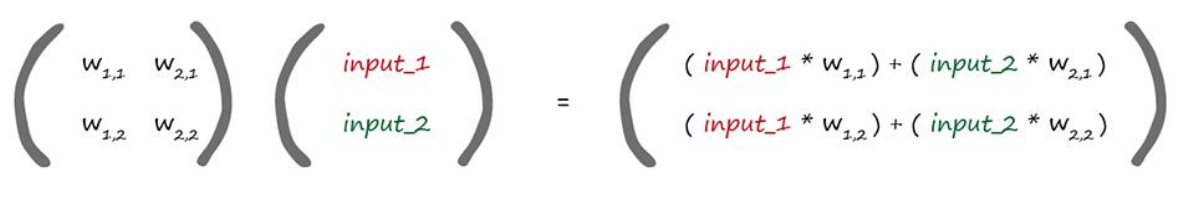
\includegraphics[scale=0.155]{nn_matrix}
\vspace{0.2cm}

\justifying
  To calculate simple feedforward Neural Network is relatively easy. For each layer we just need to calculate matrix dot product between weights and inputs. Inputs in here can be input from input layer or output from hidden layer. \cite{tariq2016}

\centering
\vspace{0.2cm}
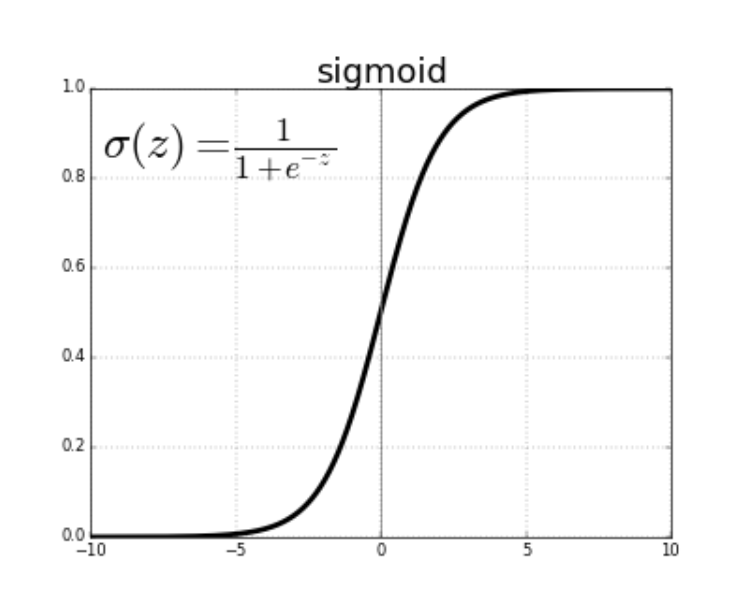
\includegraphics[scale=0.55]{sigmoid}
\vspace{0.2cm}

\justifying
  Sigmoid function is an activation function that will produce output positive number between 0 and 1. Same as the produced output, the input of the sigmoid function is better when it is between 0 and 1 too, this is the reasons we do normalization in our data before training neural network. After matrix dot calculation, before continue to the next layer, each of the element from the dot product output should be mapped to the sigmoid function. \cite{sibi2013} 

\centering
\vspace{0.2cm}
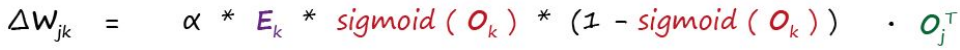
\includegraphics[scale=0.2]{delta_w}
\vspace{0.2cm}

\justifying
  Backpropagation in Artificial Neural Network is the model ability to propagate the error that it got from the differences between output and the expected output to the architectural structure of the network. The purpose of backpropagation is to update weight and bias based on the evaluated error so the network could improve its accuracy for every backpropagation. The formula above is to update the weight after all the error evaluation process. \cite{erb1993}

\section{Materials and Methods}
The dataset that we used in this paper is Medical Cost Personal Datasets from Kaggle. This dataset contains data of insurance cost factors that affect charges from health insurance company. This dataset has seven columns and 1338 rows, the name of the column and its description are:
  \begin{itemize}
    \item age: Age of primary beneficiary.
    \item sex: Insurance contractor gender (female/male).
    \item bmi: Body Mass Index, providing an understanding of body, weights that are relatively high or low relative to height, objective index of body weight (kg/m\textsuperscript{2}) using the ratio of height to weight, ideally 18.5 to 24.9. 
    \item children: Number of children covered by health insurance / Number of dependents.
    \item smoker: An active smoker or not.
    \item region: The beneficiary's residential area in the US (northeast, southeast, southwest, northwest).
    \item charges: Individual medical cost billed by health insurance.
  \end{itemize}

  Before we proceed to use the dataset to predict the healthcare cost, the first thing we need to do is a data preprocessing. Let us assume that we have already load the data from csv (comma separated value) file into the pandas dataframe. Data preprocessing is required in this pre analysis process to ensure that the data used in the analysis process is clean and has a high usability.  

\centering
\vspace{0.2cm}
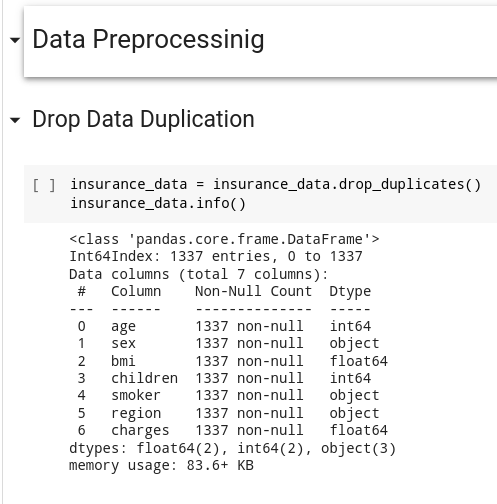
\includegraphics[scale=0.35]{drop_data_duplication}
\vspace{0.2cm}

\justifying
Data duplication is not good in analysis process. The duplicate data will need an extra time to process because we do the same thing more than once. Fortunately, pandas dataframe provides such a nice built in function to drop the duplicated data. At first we have 1338 data, after dropping the duplicated data, we left out with 1337 rows of data. 

\centering
\vspace{0.2cm}
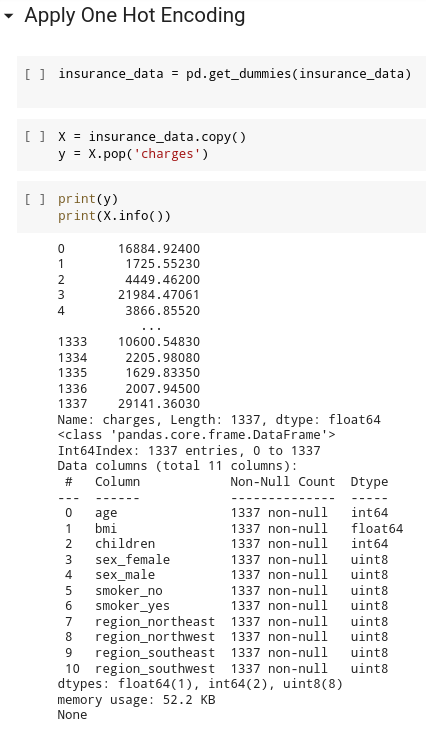
\includegraphics[scale=0.4]{one_hot_encoding}
\vspace{0.2cm}

\justifying
To process data with an Artificial Neural Network, the data must be numeric. Because the dataset that we have have a non-numeric column, so we must convert them into a numeric type. We use one-hot encoding to encode the data into numeric form because one-hot encoding is so verbose despite it will make the data dimension bigger. The expansion of the data dimension is not a problem because we only have a small data to analyze. Pandas dataframe provides the function to automatically encode the
  non-numeric column into the numeric one and drop the original column.

\centering
\vspace{0.2cm}
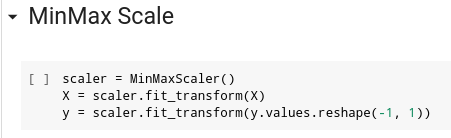
\includegraphics[scale=0.4]{min-max}
\vspace{0.2cm}

\justifying
Artificial Neural Network especially that uses the sigmoid activation function will not work well when the input data is too large. To solve this problem we use MinMaxScaler class from Scikit-Learn. \cite{sklearn_api} This will scale the data in the range from 0 to 1.

\centering
\vspace{0.2cm}
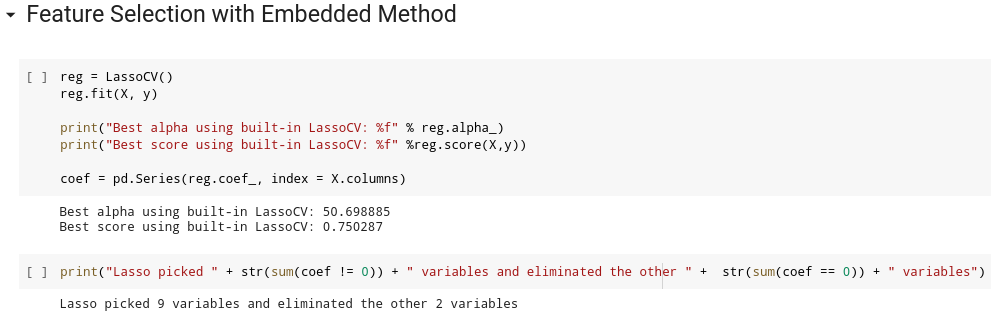
\includegraphics[scale=0.185]{feature_selection_1}
\vspace{0.2cm}

\justifying
The embedded feature selection above uses Lasso to perform the feature selection. Lasso is a machine learning algorithm so the way it is to select the important feature is through a learning. It shows that the algorithm succesfully select 9 important features and eliminated 2 uncorellated features.

\centering
\vspace{0.2cm}
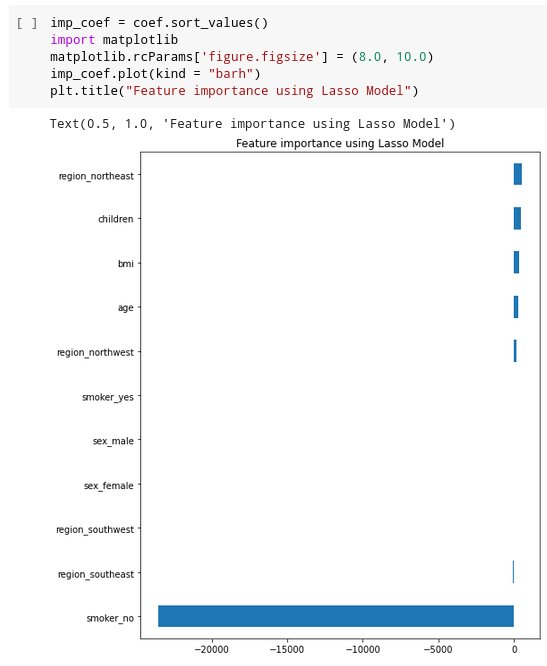
\includegraphics[scale=0.33]{feature_selection_2}
\vspace{0.2cm}

\justifying
The above picture shows that correlation coefficient for each features. As we can see, there is three feature that do not have the bar. It means that they either have a very low correlation with the dependent variable or just no correlation at all.

\centering
\vspace{0.2cm}
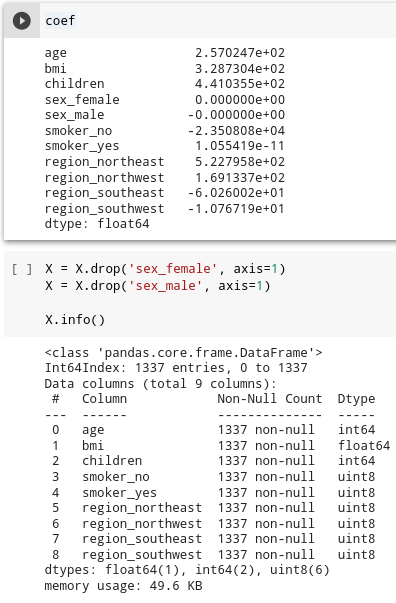
\includegraphics[scale=0.45]{feature_selection_3}
\vspace{0.2cm}

\justifying
The picture above shows that sex\_female and sex\_male have no correlation to the dependent variable. With that information we can decide to drop off both the sex\_female and sex\_male column for good. By doing this way, the data analysis will be much more efficient.

\centering
\vspace{0.2cm}
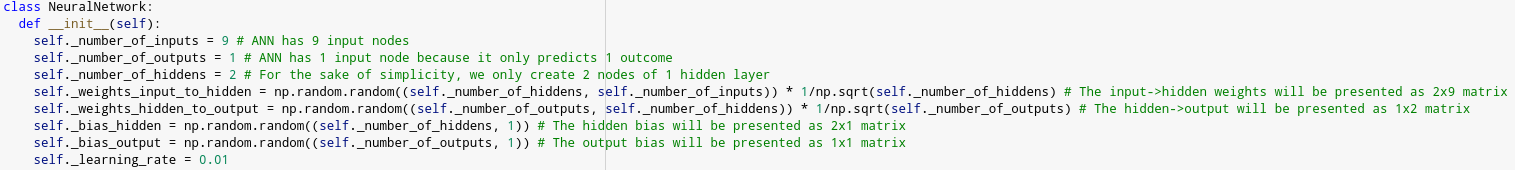
\includegraphics[scale=0.125]{nn_1}
\vspace{0.2cm}

\justifying
First thing first, we initialize the neural network class like the picture above. It has fix number of input nodes, output nodes, hidden nodes, and learning rate for the sake of simplicity. Notice that weights and bias are randomly generated, and for the weigths, they have this equation:
\begin{equation} 
  \frac{1}{\sqrt{number of hidden or output node}} 
\end{equation}
this equation make sure that the weights have the initial random number that not too far from the right final weight.

\centering
\vspace{0.2cm}
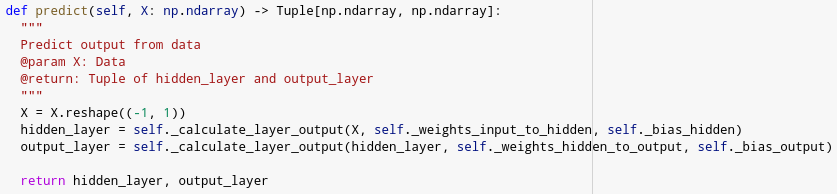
\includegraphics[scale=0.225]{nn_2}
\vspace{0.2cm}

\justifying
The predict() function will take a dataset and return the final calculation from hidden and output layer. Before being calculated, the input dataset will be reshaped to (9,2) matrix. Function that handle the calculations is \_calculate\_layer\_output(), it handle both hidden and output layer. 

\centering
\vspace{0.2cm}
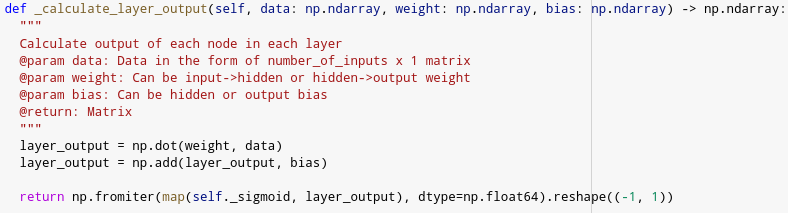
\includegraphics[scale=0.25]{nn_3}
\vspace{0.2cm}

\justifying
This is function that handles the matrix manipulation like calculate the dot product between weight and input and also add the calculation result with bias. It can handle both for hidden and output layer. The purpose of this function is to implement the DRY principle (Don't Repeat Yourself) so it can be reused in the predict() function to calculate both fot hidden and output layer. The final calculation in this function is at the return statement, it will map sigmoid function to every
member of matrix, the result from dot product and addition above it, and then convert them to the numpy array.

\centering
\vspace{0.2cm}
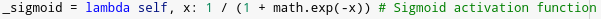
\includegraphics[scale=0.315]{nn_4}
\vspace{0.2cm}

\justifying
This is the activation function. We use sigmoid in this case because it's simple and widely use in another neural network project. The implementation in this code base is with lambda expression to save a lot of lines.

\centering
\vspace{0.2cm}
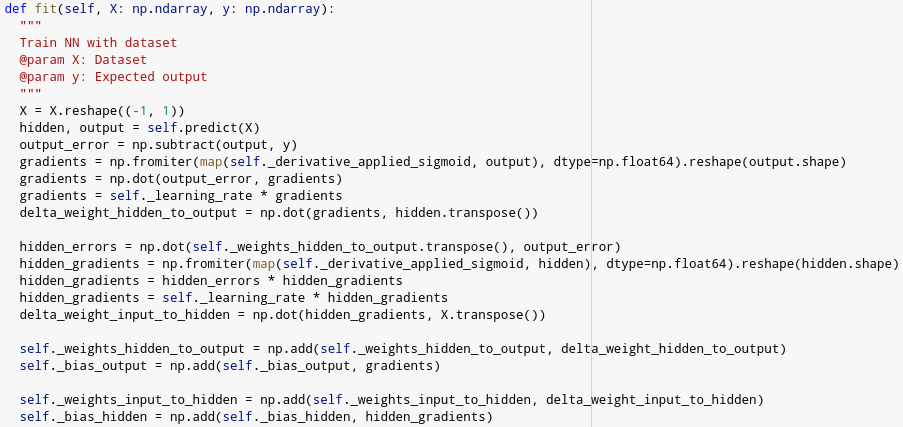
\includegraphics[scale=0.21]{nn_5}
\vspace{0.2cm}

\justifying
The fit() function is where the backpropagation begin. Basically it is just a step-by-step implementation of the delta weight function before. First thing first is call the predict() function to get the hidden and output value. Now calculate the error by subtract them. To minimize the error, we use stohastic gradient decent, the formula is actualy the derivative of sigmoid function that mapped to every member of output matrix. now calculate the dot product between error and the
gradient itself. After that multiply gradient with the learning rate, this is required so when descending the gradient, we can specify how much we want to descent. Now calculate the delta weight by do a dot product operation to gradients and tansposed hidden matrix. After that we can add the delta weight to the current weight and add gradient to the current bias. This apply both for output and input layer. After we finish, now the weight and bias is updated with the new value that we
hope can improve the prediction.

\centering
\vspace{0.2cm}
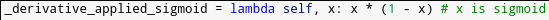
\includegraphics[scale=0.35]{nn_7}
\vspace{0.2cm}

\justifying
This is not a legit derivative of sigmoid function. We made it the way it is right now is because we already calculate the sigmoid in the predict() function. So to make everything simple, we can just simply pass the sigmoided value to this anonymous function directly.

\centering
\vspace{0.2cm}
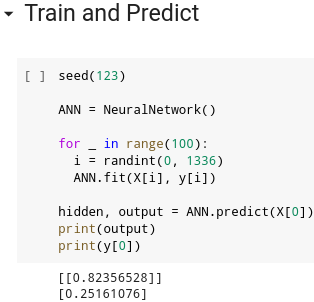
\includegraphics[scale=0.55]{nn_8}
\vspace{0.2cm}

\justifying
The last part is to training and testing the model. We train the model 100 times, each iteration we randomly select the dataset except the first data so the model will not overfit. After the training finished, we try to predict the charges with the first row dataset to verify if the model is successfuly predict the charges.

\section{Result and Conclusion}
The result from the experiment is not too good. As we can see that our model failed to predict the correct value. The difference between the output and the expected output is quite high too.

The conclusion from this experiment is that the model is failed to predict the correct charges value. The expectect value is 0.25161076 and the actual value is 0.82356528. The difference between the output and the expected output concludes that this experiment failed.
\section{Discussion}
This model can have a further improvement, despite being the failed experiment, by tunning this model with the more complex architecture, adjust learning rate, change the loss function, hopefully we can improve the performance of the model. The data also have a big portion to determine wether the model will success or not, the quality and the quantity of the data will make a big improvement because there is a principle Garbage In Garbage Out, so the data must have a good quality and good
amount of quantity too. Overall this model is still have many flaws that we can fix in the future because we do not have many time left.

\end{multicols}
\newpage
\centering
\printbibliography
\end{document}
